\subsection{Platform Initialization \gls{pi} Boot Sequence}
PI compliant system firmware must support the six phases: security (\gls{sec}), pre-efi initialization (\gls{pei}), driver execution environment (\gls{dxe}), boot device selection (\gls{bds}), run time (RT) services and After Life (transition from the OS back to the firmware) of system. Refer to Figure \ref{fig:design-pi-boot-phases} below.

\begin{figure}[h]
	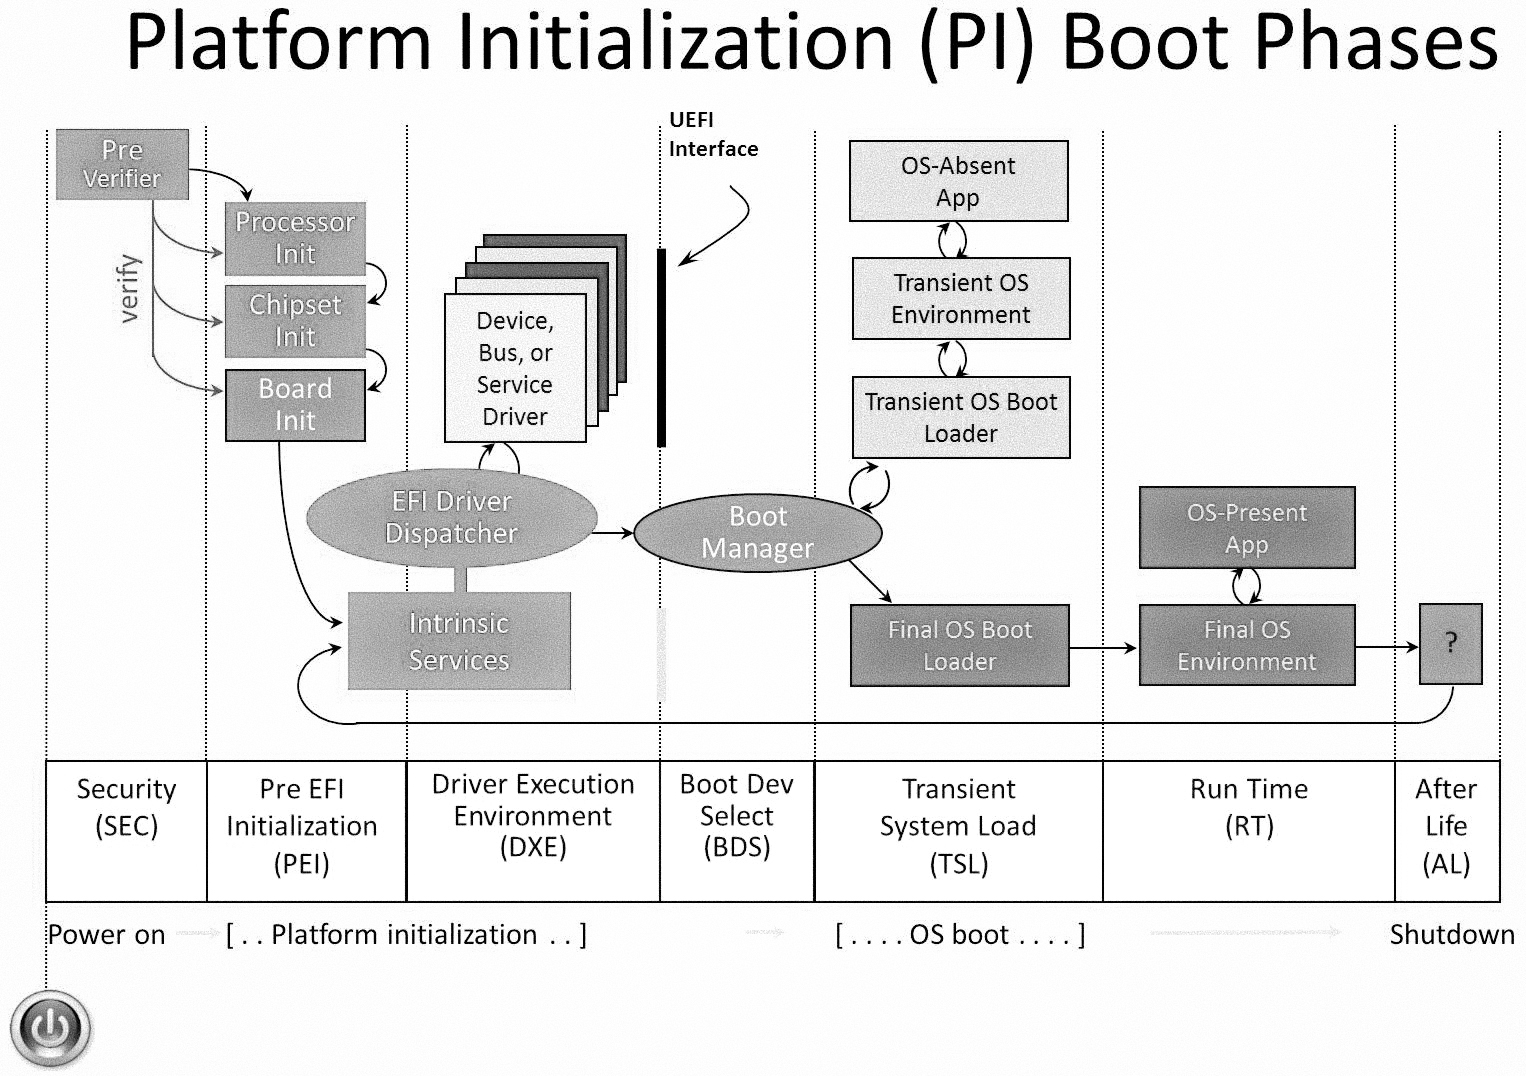
\includegraphics[width=\linewidth]{PI_Boot_Phases}
	\caption{\gls{pi} Boot Phases}\label{fig:design-pi-boot-phases}
\end{figure}

\subsection{Security (\gls{sec})}
The Security (SEC) phase is the first phase in the PI Architecture and is responsible for the following:
\begin{itemize}
	\item Handling all platform restart events
	\item Creating a temporary memory store
	\item Serving as the root of trust in the system
	\item Passing handoff information to the PEI Foundation
\end{itemize}
The security section may contain modules with code written in assembly. Therefore, some EDK II module development environment (MDE) modules may contain assembly code. Where this occurs, both Windows and GCC versions of assembly code are provided in different files

\subsection{Pre-EFI Initialization (\gls{pei})}
The Pre-EFI Initialization (PEI) phase described in the PI Architecture specifications is invoked quite betimes in the boot period. Specifically, after about preliminary processing in the Security (SEC) phase, any machine restart event will invoke the PEI phase.
The PEI phase is designed to be developed in many parts and consists of:
\begin{itemize}
	\item PEI Foundation (core code)
	\item Pre-EFI Initialization Modules (specialized plug-ins)
\end{itemize}
The PEI phase initially operates with the platform in a nascent state, leveraging only on-processor resources, such as the processor cache as a call stack, to dispatch Pre-EFI Initialization Modules (PEIMs).

The PEI phase cannot assume the availability of amounts of memory (RAM) as DXE and hence PEI phase limits its support to the following:
\begin{itemize}
	\item Locating and validating PEIMs
	\item Dispatching PEIMs
	\item Facilitating communication between PEIMs
	\item Providing handoff data to later phases
\end{itemize}

These PEIMs are responsible for the following:
\begin{itemize}
	\item Initializing some permanent memory complement
	\item Describing the memory in Hand-Off Blocks (HOBs)
	\item Describing the firmware volume locations in HOBs
	\item Passing control into the Driver Execution Environment (DXE) phase
\end{itemize}

Figure \ref{fig:design-pei-operation-diagram} shows a diagram describes the action carried out during the PEI phase

\begin{figure}[h]
	\centering
	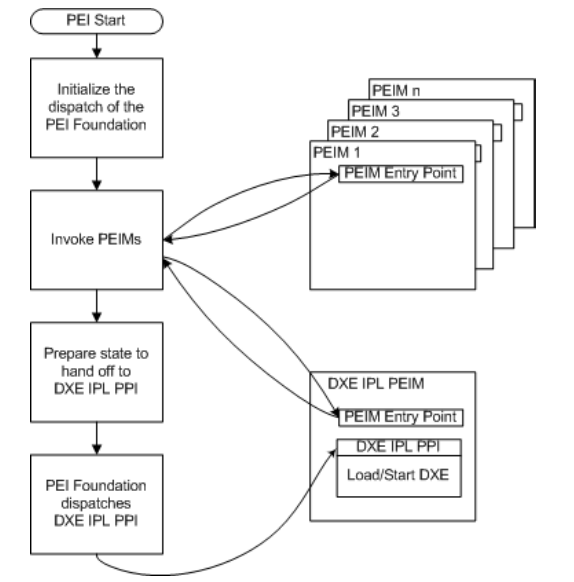
\includegraphics[width=0.7\linewidth]{design/pei-operation-diagram}
	\caption{Diagram of PI Operations}\label{fig:design-pei-operation-diagram}
\end{figure}

\subsubsection{PEI Services}
The PEI Foundation establishes a system table named the PEI Services Table that is visible to all Pre-EFI Initialization Modules (PEIMs) in the system. A PEI Service is defined as a function, command, or other capability manifested by the PEI Foundation when that service’s initialization requirements are met. Because the PEI phase has no permanent memory available until nearly the end of the phase, the range of services created during the PEI phase cannot be as rich as those created during later phases. Because the location of the PEI Foundation and its temporary RAM is not known at build time, a pointer to the PEI Services Table is passed into each PEIM’s entry point and also to part of each PEIM-to-PEIM Interface (PPI). 

The PEI Foundation provides the classes of services listed in Table \ref{table:design-pei-foundation-class-service}

\begin{table}[h]
	\centering
	\begin{tabular}{ l | p{8cm} }
		Service & Details
		\\ \hline \hline
		PPI Services & Manages PPIs to ease inter-module method calls between PEIMs. A database maintained in temporary RAM to track installed interfaces.
		\\ \hline
		Boot Mode Services & Manages the boot mode (S3, S5, diagnostics, normal boot, etc.)
		\\ \hline
		HOB Services & Creates data structures (Hand-off-blocks) that are used to convey information to the next phase 
		\\ \hline
		Firmware Volume Services & Finds PEIMs and along with that other firmware files in the firmware volumes
		\\ \hline
		PEI Memory Services & provides a collection of memory management services (to be used before and after permanent memory to discovered)
		\\ \hline
		Status Code Services & Provides general progress and error code reporting services (i.e. port 080h or a serial port for text output for debug)
		\\ \hline
		Reset Services & Provides a common means to aid initializing warm or cold restart of the system
		\\ \hline
	\end{tabular}
	\caption{Services provided by PEI Foundation Classes}\label{table:design-pei-foundation-class-service}
\end{table}


\subsubsection{PEI Foundation}
The PEI Foundation is the entity that carried outs following activity:
\begin{itemize}
	\item Dispatching of Pre-EFI initialization modules (PEIMs)
	\item Maintaining the boot mode
	\item Initialization of permanent memory
	\item Invoking the DXE loader 
\end{itemize}
The PEI Foundation written to be portable across all the various platforms architecture of a given instruction-set. i.e. A binary for IA-32 (32-bit Intel architecture) works across all Pentium processors and similarly Itanium processor family work across all Itanium processors.

Irrespective of the processor micro architecture, the set of services uncovered by the PEI Foundation should be the same. This consistent surface area around the PEI Foundation allows PEIMs to be written in the $C\ programming\ language$ and compiled across any micro architecture.

\subsection{PEI Dispatcher}
The PEI Dispatcher is basically a state machine which is implemented in the PEI Foundation. The PEI Dispatcher evaluates the dependency expressions in Pre-EFI initialization modules (PEIMs) that are lying in the \gls{fv}s being examined.

Dependency expressions are coherent combinations of PEIM-to-PEIM Interfaces (PPIs). These expressions distinguish the PPIs that must be available for use before a given PEIM can be invoked. The PEI Dispatcher references the PPI database in the PEI Foundation to conclude which PPIs have to be installed and evaluate the dependency expression for the PEIM. If PPI has already been installed then dependency expression will evaluate to $TRUE$, which notifies  PEI Dispatcher it can run PEIM. At this stage, the PEI Foundation handovers control to the PEIM with $TRUE$ dependency expression. 

The PEI Dispatcher will exit Once the PEI Dispatcher has examined and evaluated all of the PEIMs in all of the uncovered firmware volumes and no more PEIMs can be dispatched (i.e. the dependency expressions do not evaluate from $FALSE$ to $TRUE$). At this stage, the PEI Dispatcher cannot invoke any additional PEIMs. The PEI Foundation then takes back control from the PEI Dispatcher and invokes the $DXE IPL PPI$ to pass control to the DXE phase of execution.

\subsection{Drive Execution Environment (\gls{dxe})}
Prior to the DXE phase, the Pre-EFI Initialization (PEI) phase is responsible for initializing permanent memory in the platform so that the DXE phase can be loaded and executed. The state of the system at the end of the PEI phase is passed to the DXE phase through a list of position independent data structures called Hand-Off Blocks (HOBs). HOBs are described in detail in the Platform Initialization Specification.
There are several components in the DXE phase:
\begin{itemize}
	\item DXE Foundation
	\item DXE Dispatcher
	\item A set of DXE Drivers
\end{itemize}

\subsection{Boot Device Selection (\gls{bds})}
The Boot Device Selection (BDS) phase is implemented as part of the BDS Architectural Protocol. The DXE Foundation will hand control to the BDS Architectural Protocol after all of the DXE drivers whose dependencies have been satisfied have been loaded and executed by the DXE Dispatcher. The BDS phase is responsible for the following:
\begin{itemize}
	\item Initializing console devices
	\item Loading device drivers
	\item Attempting to load and execute boot selections
\end{itemize}

\subsection{Transient System Load (TSL) and Runtime (RT)}
The Transient System Load (TSL) is primarily the OS vendor provided boot loader. Both the TSL and the Runtime Services (RT) phases may allow access to persistent content, via UEFI drivers and UEFI applications. Drivers in this category include PCI Option ROMs.

\subsection{After Life (AL)}
The After Life (AL) phase consists of persistent UEFI drivers used for storing the state of the system during the OS orderly shutdown, sleep, hibernate or restart processes.

